\chapter*{Deliberate Discovery with Examples}

\ifcontent

    Using examples to actively find out what you don't know.

\fi 

\section*{Discovery using examples}

\ifnotes

    Learning outcomes:
    
    \begin{itemize}
        \item Create concrete examples - containing action \& outcome
        \item Identify missing rules and/or assumptions
    \end{itemize}

    Write attendees' assumptions up on the whiteboard, in two columns. One for assumptions about rules, another one for assumptions about context. Ask attendees if they can guess why you created two columns. If not, explain. Rules always apply, regardless of context. Context only applies to individual examples.
    
    Attendees often say there are too many unknowns to start. Push back on this. Ask: Do we know enough to start defining the interface of a function? For example billsDispensed(billInventory, requestedAmount) -> Map<Denomination,Count>. Can we develop something that does this even if we lack all knowledge about rules? (Yes we can)
    
\fi

\ifcontent

    Imagine you're developing software for an ATM that dispenses \$10, \$20 and \$50 bills. Consider this user story:
    
    
    \begin{center}
    \begin{varwidth}{\columnwidth}
    \begin{verbatim}
    As a checking account customer
    I want to receive a mix of bills when I withdraw cash from an ATM
    So that I don't have to rely on vendors being able to break large bills
    \end{verbatim}
    \end{varwidth}
    \end{center}
    
    
    At your table start creating examples that demonstrate how your ATM software meets the needs of the checking account customer described in this story. Consider what bills should be dispensed when the customer requests different amounts of cash.
    
    Write each example on a separate green index card. Follow the format of the following three example cards:
    
    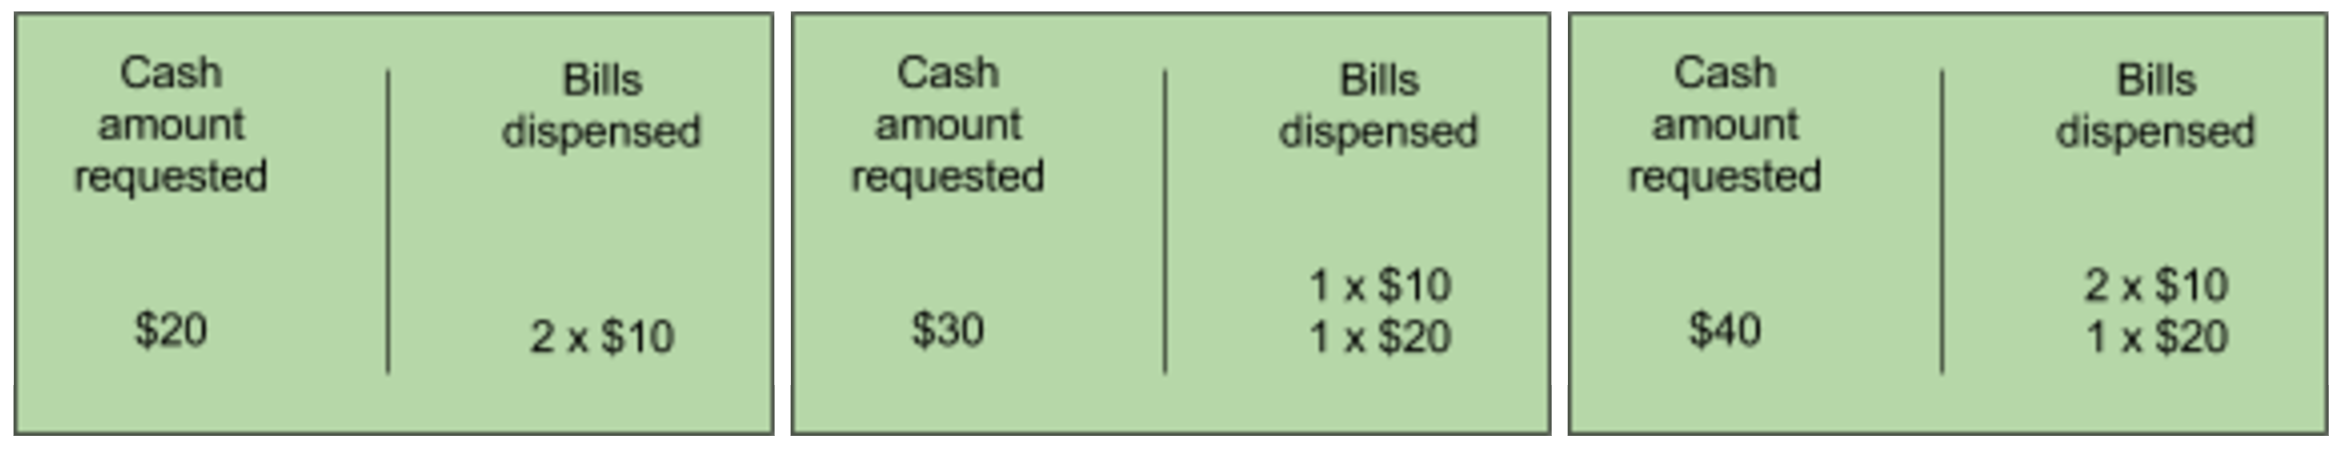
\includegraphics[width=\textwidth]{images/atm-example-without-context}
    
    \QandAbox{What questions did you have to answer to be able to come up with these examples?}{1.5}
    
    \QandAbox{Have you got enough examples to start development? Or do you need more?}{1.5}
    

    \QandAbox{Which came first, example or rule?}{1.5}

\fi

\chapter*{Context - Action - Outcome}
    
\ifnotes

    The content of this section is important, but the actual activity can be skipped. Some tables might have already created examples that need the ATM to run out of bills (or have a network failure or power outage)
    
    \begin{itemize}
        \item Define examples as being made up of context, action, outcome
        \item Explain why, in some situations, the context should be left implicit.
    \end{itemize}

    Implicit context: Ask - "How often do you go to get cash out of an ATM and wonder to yourself 'I hope the ATM has cash in it'?" The answer is "never" - this is an implicit context. Requirements \& documentation should be read, so we need to omit implicit, inessential information.

    This is a good time to introduce Context Questions and Outcome Questions. 1) Pick an example and change the context so that the outcome is different (keep action unchanged). 2) Pick an example and talk about additional outcomes that you haven't listed. (Return card, update bill inventory, debit account, print receipt etc.)
\fi

\ifcontent

    The ATM examples you created earlier described an action ("Cash amount requested") and an outcome ("Bills dispensed"). There's often a context to consider too:
    
    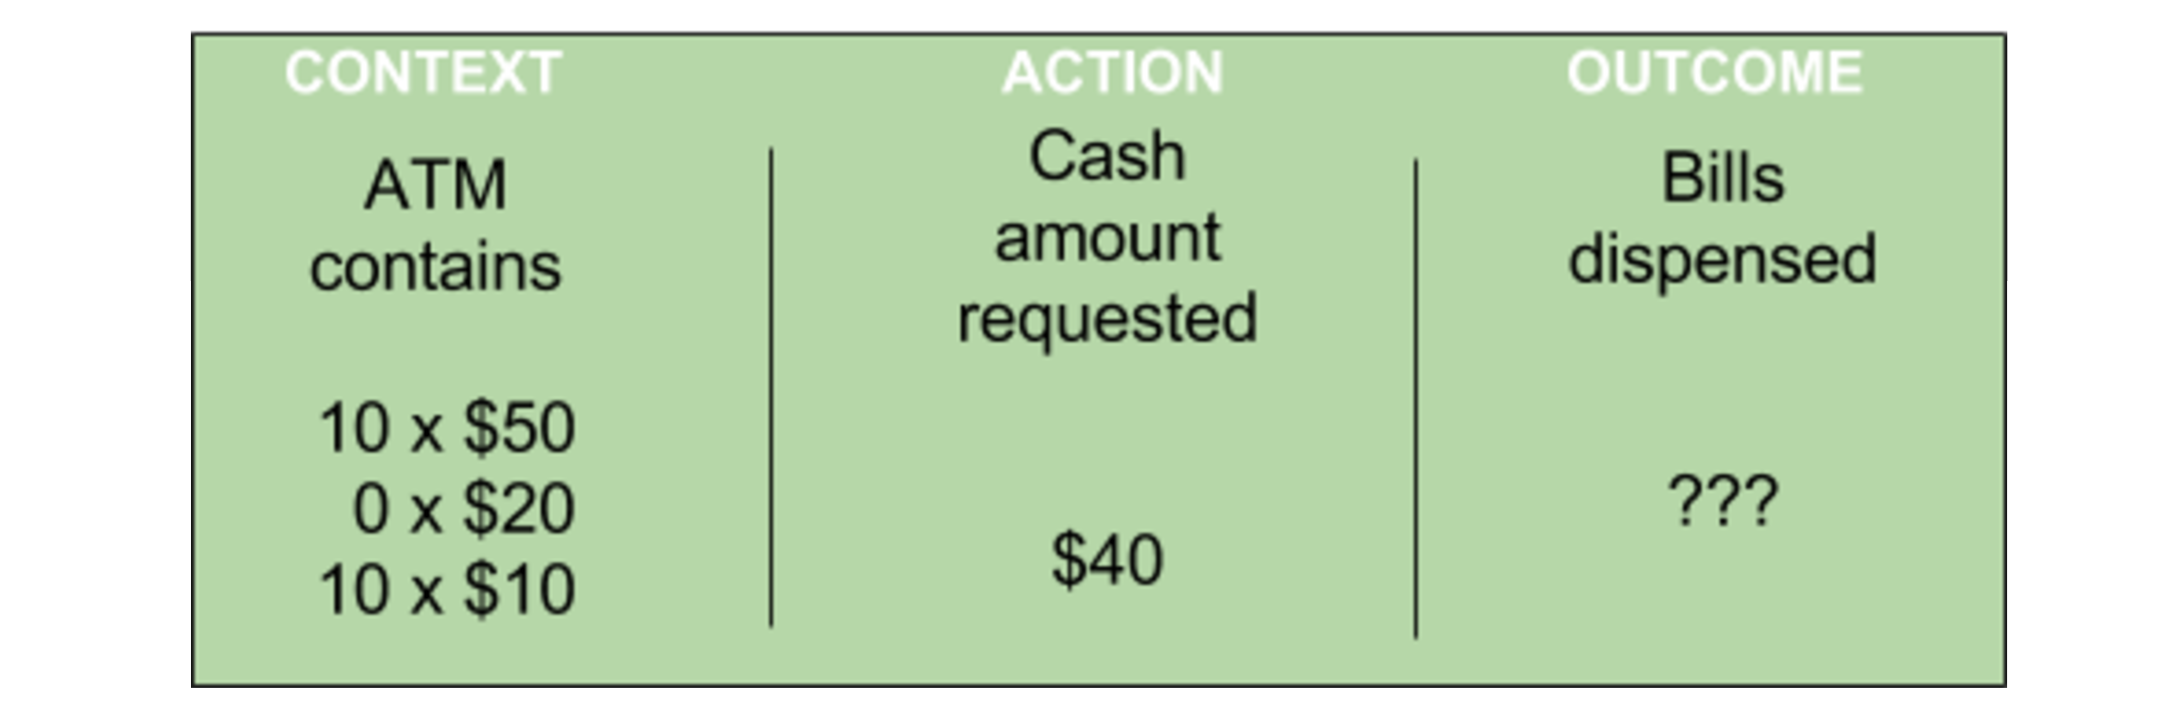
\includegraphics[width=\textwidth]{images/atm-example-with-context}
    
    \QandAbox{Look back at the examples that you have already created. Do any of them already describe a context? If not, what are their \emph{implicit} contexts?}{5}

\fi